\newpage
\chapter{Комуникация клиент-сървър}
\label{chapter06}

Комуникацията между Android клиента и PHP базирания сървър се извършва през HTTP с размяна на JSON пакетирани съобщения. 

\section{Hypertext Transfer Protocol}

При всяко създаване на инстанция за тапета е нужно да се извърши свързване към отдалечения сървър и да бъде заявен пакет за работа. Ако връзката не е възможна се използват данните записани в локалната база данни. 

\begin{figure}[h]
  \centering
  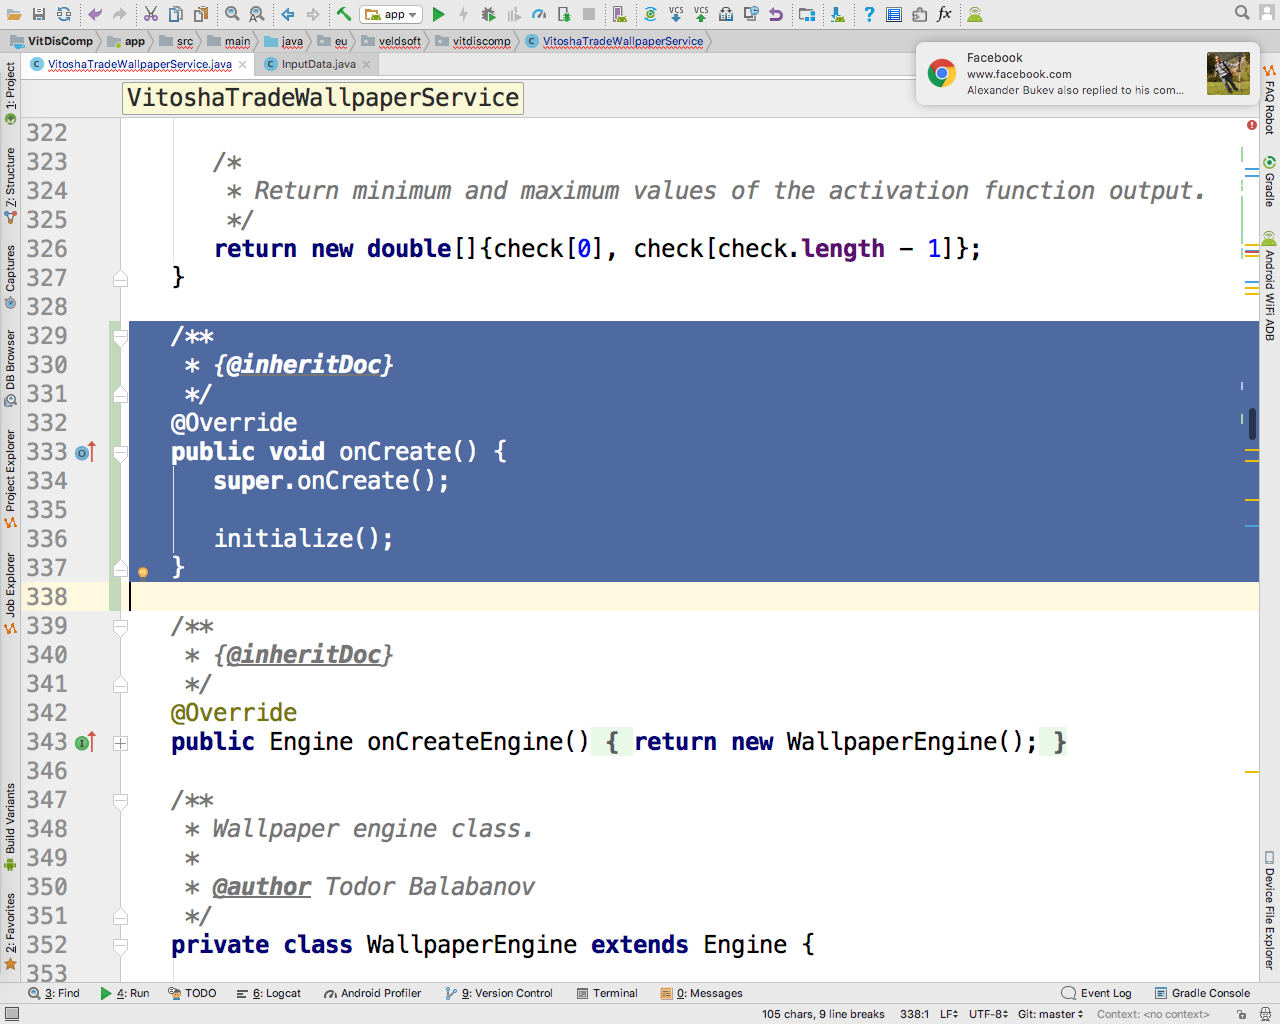
\includegraphics[height=0.45\pdfpageheight]{pic0155}
  \caption{Инициализация на вътрешните променливи.}
\label{fig:pic0155}
\end{figure}
\FloatBarrier

Инициализацията на вътрешните променливи се осъществява в събитието onCreate (Фиг. \ref{fig:pic0155}).

\begin{figure}[h]
  \centering
  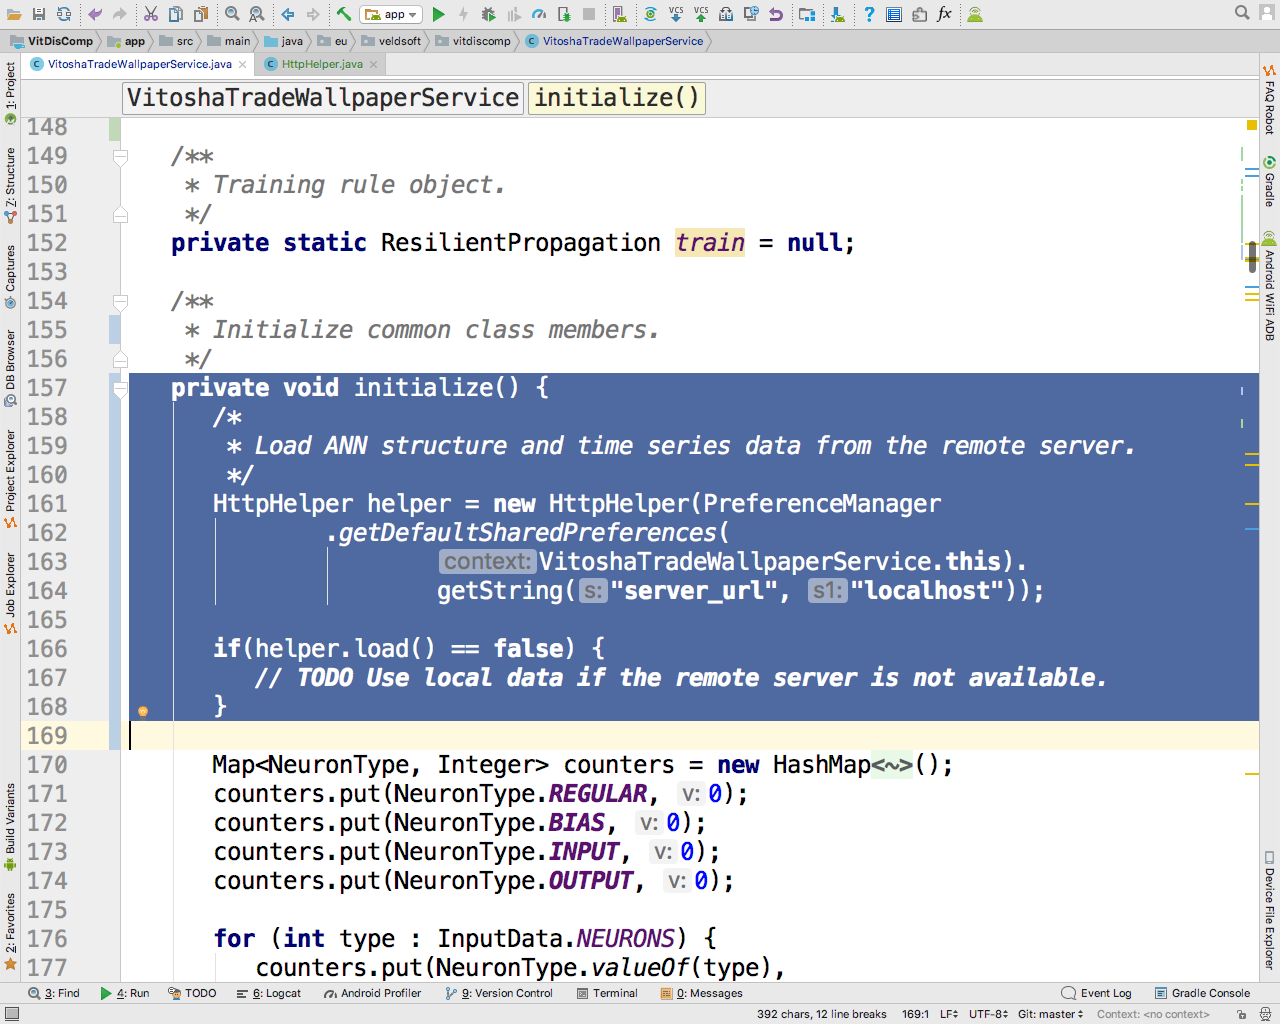
\includegraphics[height=0.45\pdfpageheight]{pic0156}
  \caption{Зареждане на данните с помоща на HTTP комуникация.}
\label{fig:pic0156}
\end{figure}
\FloatBarrier

Инициализирането на вътрешните променливи през HTTP се поема от допълнително създаден, помощен обект, който е от клас отговорен за комуникацията (Фиг. \ref{fig:pic0156}). 

\section{JavaScript Object Notation}
